% https://tex.stackexchange.com/questions/80502/how-to-draw-a-3d-curved-manifold-in-tikz

\documentclass[border=5pt, multi, tikz]{standalone}
\usepackage{tikz}
\usepackage{amsmath}
\usetikzlibrary{intersections,shapes.arrows}

\newcommand\Dist[1]{\phantom{\rule{#1}{4pt}}}

\usepackage{xcolor}

% Define colors
\definecolor{myred}{RGB}{255,0,0}
\definecolor{myblue}{RGB}{0,0,255}
\definecolor{mygreen}{RGB}{0,255,0}
\definecolor{mypurple}{RGB}{128,0,128}


\definecolor{forestgreen(web)}{rgb}{0.13, 0.55, 0.13}

\begin{document}

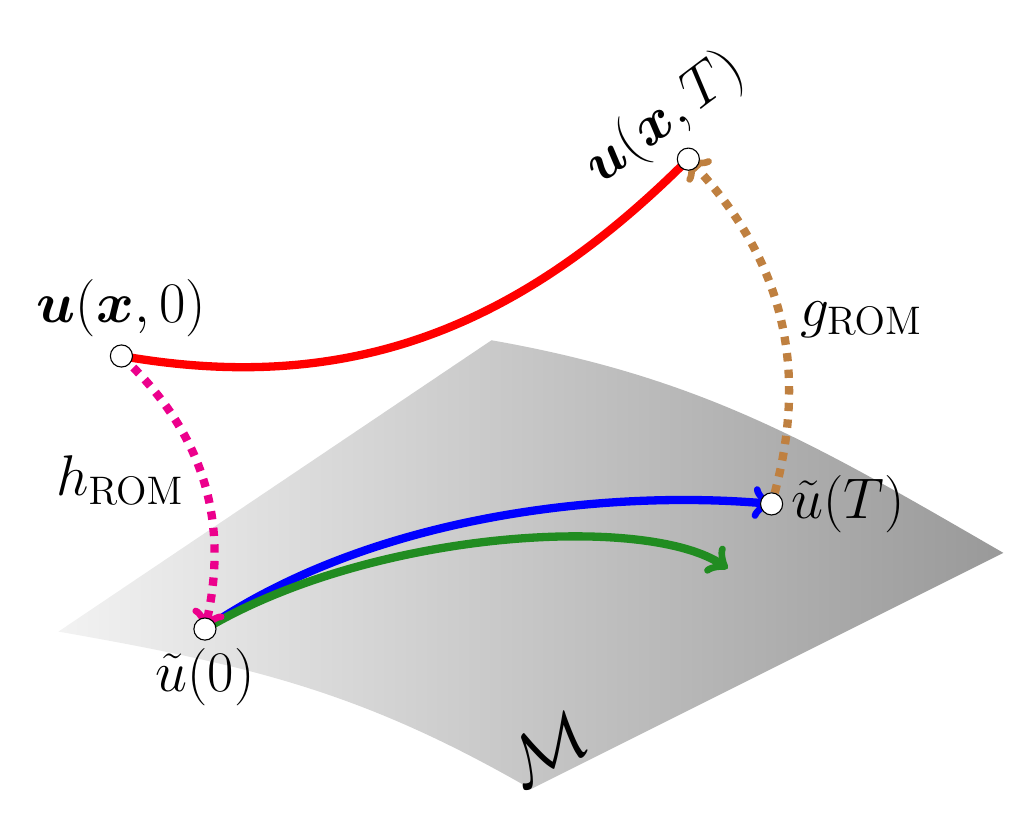
\begin{tikzpicture}

% the bottom left border of the surface
\path[name path=border1] (0,0) to[out=-10,in=150] (6,-2);
% the upper right border of the surface
\path[name path=border2] (12,1) to[out=150,in=-10] (5.5,3.2);
% a path for a line crossing both borders
\path[name path=blueline] (0,-0.4) -- (12,1.5);
% intersections between the borders and the lines
\path[name intersections={of=border1 and blueline,by={a}}];
\path[name intersections={of=border2 and blueline,by={b}}];

%% we draw the surface
\shade[left color=gray!10,right color=gray!80] 
  (0,0) to[out=-10,in=150] (6,-2) -- (12,1) to[out=150,in=-10] (5.5,3.7) -- cycle;

\draw[red, line width=3.0pt] (0.8,3.5) to[out=-10,in=225] 
  coordinate[pos=0.00] (aux1) 
  coordinate[pos=1.00] (aux3) (8,6);

\draw[draw = none] (a) .. controls (6,1.5) and (7,2) .. 
  coordinate[pos=0.05] (bux1) 
  coordinate[pos=0.8] (bux3) (b);

\draw[blue, ->, line width = 3.0pt] (bux1) .. controls (4,1.5) and (7,1.8) .. 
  (bux3);

% green curve that deviates from the blue curve
\draw[forestgreen(web), line width = 3.0pt, ->] (bux1) .. controls (4,1.3) and (7.5,1.5) .. 
  (8.5,0.8);

% we draw the dashed lines from the curved line on top to the solid line on surface
%\foreach \coor in {1,3}
%  \draw[dashed, ->, line width = 3.0pt] (aux\coor)to[bend left] (bux\coor);
  
% \draw[preaction={draw=black, line width=3.5pt, dashed}, draw=black, dashed, line width = 3.0pt] (aux1)to[bend left] coordinate[pos=0.5] (lux1) (bux1);
% \draw[preaction={draw=black, line width=3.5pt, dashed}, draw=black, dashed, line width = 3.0pt] (aux3)to[bend left] coordinate[pos=0.5] (lux2) (bux3);

\draw[magenta, dashed, ->, line width = 3.0pt] (aux1)to[bend left] coordinate[pos=0.5] (lux1) (bux1);
\draw[brown  , dashed, <-, line width = 3.0pt] (aux3)to[bend left] coordinate[pos=0.5] (lux2) (bux3);

\node[label=left:{\huge $h_\text{ROM}$}] at (lux1) {};
\node[label=right:{\huge $g_\text{ROM}$}] at (lux2) {};


% we draw the markers on the top line and place the labels
\foreach \coor/\subs in {1/-1,3/1}
{
  \draw[fill=white] (aux\coor) circle (4pt);
  \draw[fill=white] (bux\coor) circle (4pt);
}

\node[label=above:{\huge $\boldsymbol{u}(\boldsymbol{x}, 0)$}] at (aux1) {};
\node[label={[rotate=37]above:{\huge $\boldsymbol{u}(\boldsymbol{x}, T)$}}] at (aux3) {};

\node[label=below:{\huge $\tilde{u}(0)$}] at (bux1) {};
\node[label=right:{\huge $\tilde{u}(T)$}] at (bux3) {};

%% we add some labels
\node[rotate=30] at (6.2,-1.5) {\Huge $\mathcal{M}$};

%\node at ([yshift=-1cm]current bounding box.south) {
%\setlength\tabcolsep{3pt}
%\begin{tabular}{@{}cl@{\hspace{12pt}}cl@{}}
%\tikz\draw (0,0) circle (2pt); & Underlying model & \sffamily x & Prediction \\ 
%\tikz\draw[fill=red] (0,0) circle (2pt); & Filter (MAP estimate) 
%  %& \tikz\draw[fill] (0,0) circle (2pt); & MLE
%\end{tabular}
%};

\end{tikzpicture}

\end{document}